\documentclass[../../main.tex]{subfiles}

\begin{document}
\graphicspath{{imgs/}{03_firmware/imgs/}}

\chapter{Ranging layered architecture}

The ranging system is implemented follow 3 layers model as shown in figure \ref{fig:ranging_layered_architecture}. 
\begin{itemize}
    \item CCP (Clock Calibration Packet) provides synchronization service for the upper layer. All nodes jointed to the network will be synced each time a new superframe start.
    \item TDMA (Time Division Multiple Access): Each superframe is divided into multiple slots. TDMA layer provides slot service for its upper layer. 
    \item TWR (Two Way Ranging) layer runs ranging session in the time slot provided by TDMA layer.
\end{itemize}
\begin{figure}[H]
    \begin{center}
        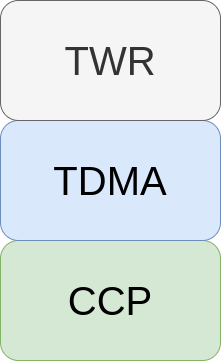
\includegraphics[scale=0.3]{ranging_layered_architecture}
    \end{center}
    \caption{Ranging layered architecture}
    \label{fig:ranging_layered_architecture}
\end{figure}

\section{Clock calibration packet (CCP)}
The main role clock calibration packet is to provide the superframe synchronization between nodes. 
\subsection{CCP role}
Three CCP roles are defined, allowing nodes to sync with others: Master, Slave, Relay.
\begin{itemize}
    \item \textbf{CCP master}: There is only and only one master node over the network. The master node is the only place where a clock calibration packet is produced. It will produce and transmit the clock calibration packet with the interval defined as a constant in the firmware. My implementation use the value of 100ms for such interval. 
    \item \textbf{CCP slave}: Slave nodes listen for the clock calibration packet to start their internal timer for each superframe.
    \item Relay: Relay nodes repeat the clock calibration packet to extend the network physical area. Before repeating the packets, they must do some modification so the receiver can sync with the  master node. There is a constraint in the maximum of repeat level which will be analyzed afterward.
\end{itemize}
\subsection{CCP packet format}

\begin{figure}[H]
    \centering
    \begin{bytefield}[bitwidth=1.1em]{32}
        \bitheader{0-31} \\
        \begin{rightwordgroup}{IEEE \\ bink frame}
            \bitbox{8}{fctrl} & 
            \bitbox{8}{seq num} & \\ 
            \bitbox{32}{euid high} \\ 
            \bitbox{32}{euid low}
        \end{rightwordgroup} \\
        \bitbox{16}{short address} &
        \bitbox{8}{} &
        \bitbox{8}{ti high} \\
        \bitbox{32}{ti low} \\
        \begin{rightwordgroup}{ccp timestamp}
            \bitbox{1}{hf} & 
            \bitbox{23}{} & 
            \bitbox{8}{timestamp high} \\ 
            \bitbox{32}{timestamp low}
        \end{rightwordgroup} \\
        \bitbox{8}{rpt count} &
        \bitbox{8}{rpt max}
        \bitbox{16}{epoch to rm us}
    \end{bytefield}
    \caption{CCP blink frame}
    \label{fig:ccp_blink_frame}
\end{figure}

\subsection{CCP master selection algorithm}
To-do

\section{Time Division Multiple Access (TDMA)}
The fundamental role of the TDMA layer is to give a notification to its upper layer when it is the time to run the service. To archive this, a node must firstly ask for getting an appropriate and available slot from jointed nodes.

\subsection{TDMA role}
In the TDMA layer, a jointed node must take one of two roles: Anchor or Tag.
\begin{itemize}
    \item TDMA Anchor: A node taking the role as an anchor must be fixed and broadcast its pre-configured location information to others.
    \item TDMA Tag: TDMA tag node is the mobile node needed to be located in the coordinate of anchors.
\end{itemize}

\subsection{TDMA slot}
The superframe is divided into multiple slots as shown in figure \ref{fig:tdma_slot}.
\begin{figure}[H]
    \begin{center}
        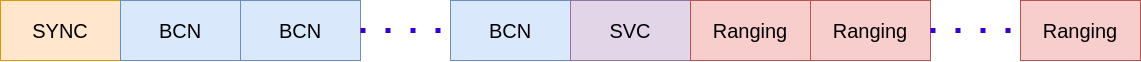
\includegraphics[scale=0.4]{tdma_slot.png}
    \end{center}
    \caption{TDMA slot}
    \label{fig:tdma_slot}
\end{figure}

\subsubsection{Synchronization slot (SYNC slot)}
In the SYNC slot interval, a master node produces and transmits the clock calibration packet. Relay nodes also repeat the clock calibration packet in this interval too.
\subsubsection{Beacon slot (BCN slot)}
An anchor node will broadcast its location and slot map information in its BCN slot. It is allowed for a jointed anchor to skip some superframes as long as it does not exceed a certain value. Other anchor nodes consider a node has left the network when they do not see any BCN message from such node for a number of superframes. The implementation uses the value of 10 for this purpose.
\subsubsection{SVC slot}
When a node wants to joint the network as a tag or anchor, it has to send its joint request in an SVC slot. The request is broadcasted and responded by all jointed anchors in their next assigned BCN slot.
\subsubsection{Ranging slot}
A jointed tag initiates the range request in its assigned ranging slot. During the remaining interval, it also listens for the response from anchors to calculate to ToF (Time of Flight).

\subsection{TDMA packet format}
The message include two parts: IEEE frame header and payload:
\begin{itemize}
    \item IEEE fame header conforms the 802.15.4-2016 standard
    \item Payload field may contain more than one message. Each message have TLV (type-length-value) format as shown in figure \ref{fig:tdma_frame_payload}. Currently, three message types are defined: \textbf{Slot request/response}, \textbf{Location}, \textbf{Slot map}. The value of these message type are illustrated in figure \ref{fig:slot_request_response_message}, \ref{fig:location_value}, \ref{fig:slot_map_message}.
\end{itemize}
\begin{figure}[H]
    \centering
    \begin{bytefield}[bitwidth=1.1em]{32}
        \bitheader{0-31} \\
        \begin{rightwordgroup}{IEEE \\ frame \\ header}
            \bitbox{16}{fctrl} & 
            \bitbox{8}{seq num} & \\ 
            \bitbox{16}{PANID} \\ 
            \bitbox{16}{dst address} &
            \bitbox{16}{src address}
        \end{rightwordgroup} \\
        \wordbox[tlr]{1}{payload} \\
        \wordbox[blr]{1}{$\cdots$}
    \end{bytefield}
    \caption{TDMA frame}
    \label{fig:tdma_frame}
\end{figure}

\begin{figure}[ht]
    \centering
    \begin{bytefield}[bitwidth=1.1em]{32}
        \bitheader{0-15}\\
        \bitbox{8}{type} & 
        \bitbox{8}{len} & 
        \bitbox{16}{value}
    \end{bytefield}
    \caption{TDMA frame payload}
    \label{fig:tdma_frame_payload}
\end{figure}

\begin{figure}[H]
    \centering
    \begin{bytefield}[bitwidth=2em]{16}
        \bitheader{0-15} \\
        \bitbox{8}{slot} &
        \bitbox{8}{slot request/response}
    \end{bytefield}
    \caption{Slot request/response message}
    \label{fig:slot_request_response_message}
\end{figure}

\begin{figure}[H]
    \centering
    \begin{bytefield}[bitwidth=1.1em]{32}
        \bitheader{0-31} \\
        \bitbox{8}{slot} \\
        \bitbox{32}{location x} \\
        \bitbox{32}{location y} \\ 
        \bitbox{32}{location z}
    \end{bytefield}
    \caption{Location message value}
    \label{fig:location_value}
\end{figure}

\begin{figure}[H]
    \centering
    \begin{bytefield}[bitwidth=1.1em]{32}
        \bitheader{0-31} \\
        \bitbox{8}{slot} \\
        \bitbox{32}{slot map high} \\
        \bitbox{32}{slot map low}
    \end{bytefield}
    \caption{Slot map message}
    \label{fig:slot_map_message}
\end{figure}

\subsection{Network management algorithm}

\subsubsection{State diagram}
The TDMA state diagram is shown in figure \ref{fig:tdma_state_diagram}. 
The master node is the initiator of the network. It has to be an anchor and occupy BCN slot 1. Since there is no jointed node before, the master node does not need to ask others. Hence, after ccp layer provides first synchronization, all nodes begin with REQT state except for the master node. 

\begin{figure}[H]
    \begin{center}
        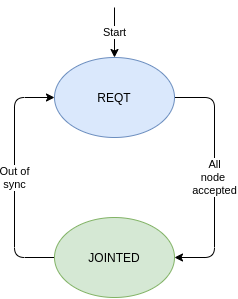
\includegraphics[scale=0.6]{tdma_state_diagram.png}
    \end{center}
    \caption{TDMA state diagram}
    \label{fig:tdma_state_diagram}
\end{figure}

\subsubsection{REQT state flow chart}
The REQT state implementation is illustrated in the follow chart \ref{fig:REQT_state_diagram}.
\begin{figure}[H]
    \begin{center}
        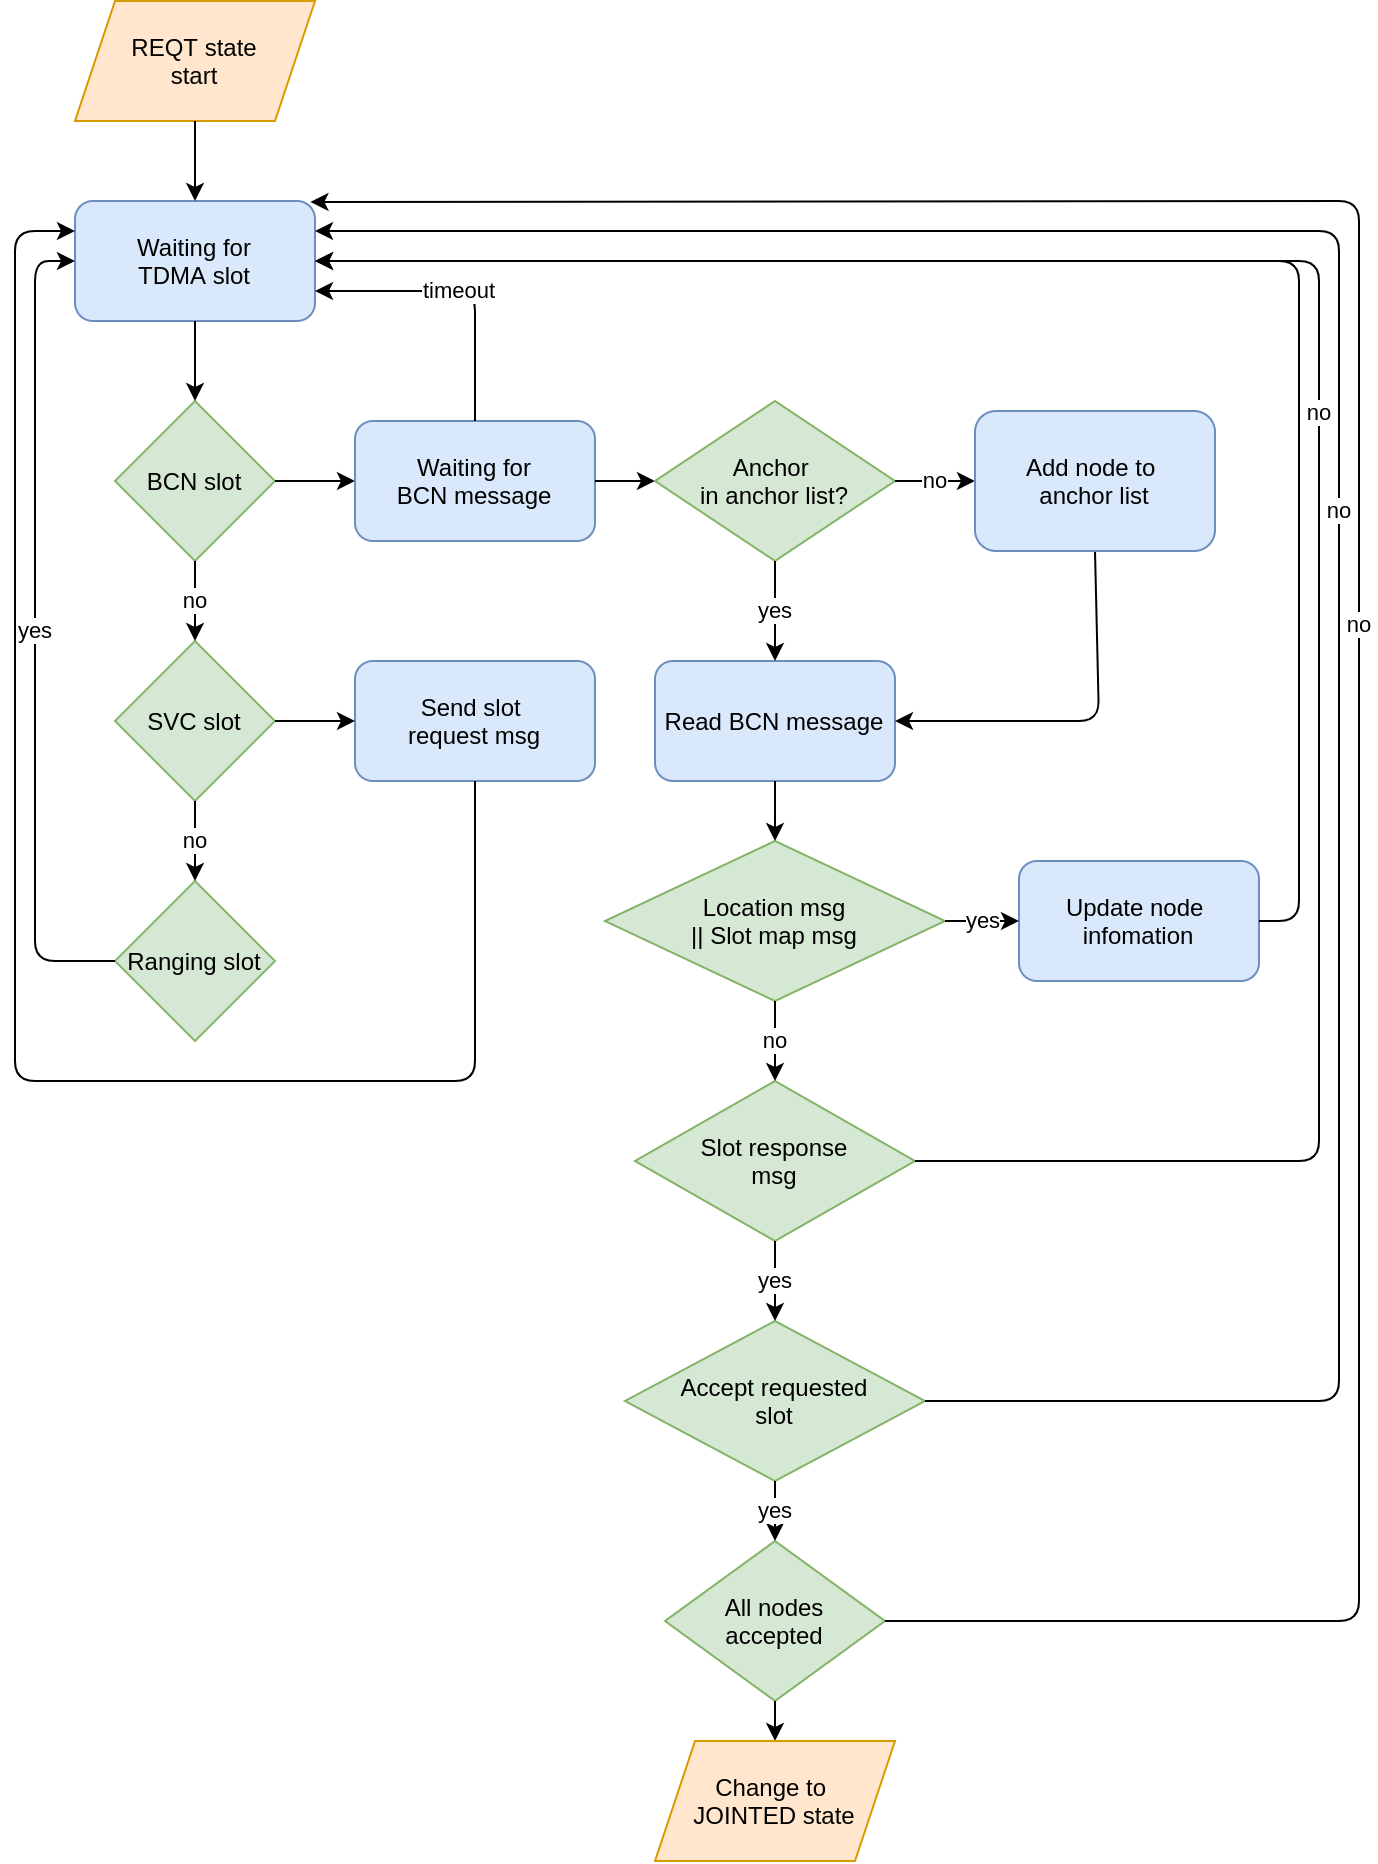
\includegraphics[scale=0.33]{REQT_flow_chart.png}
    \end{center}
    \caption{REQT state diagram}
    \label{fig:REQT_state_diagram}
\end{figure}

\subsubsection{JOINTED state flow chart}
The JOINTED state implementation is illustrated in the follow chart \ref{fig:JOINTED_state_diagram}
\begin{figure}[H]
    \begin{center}
        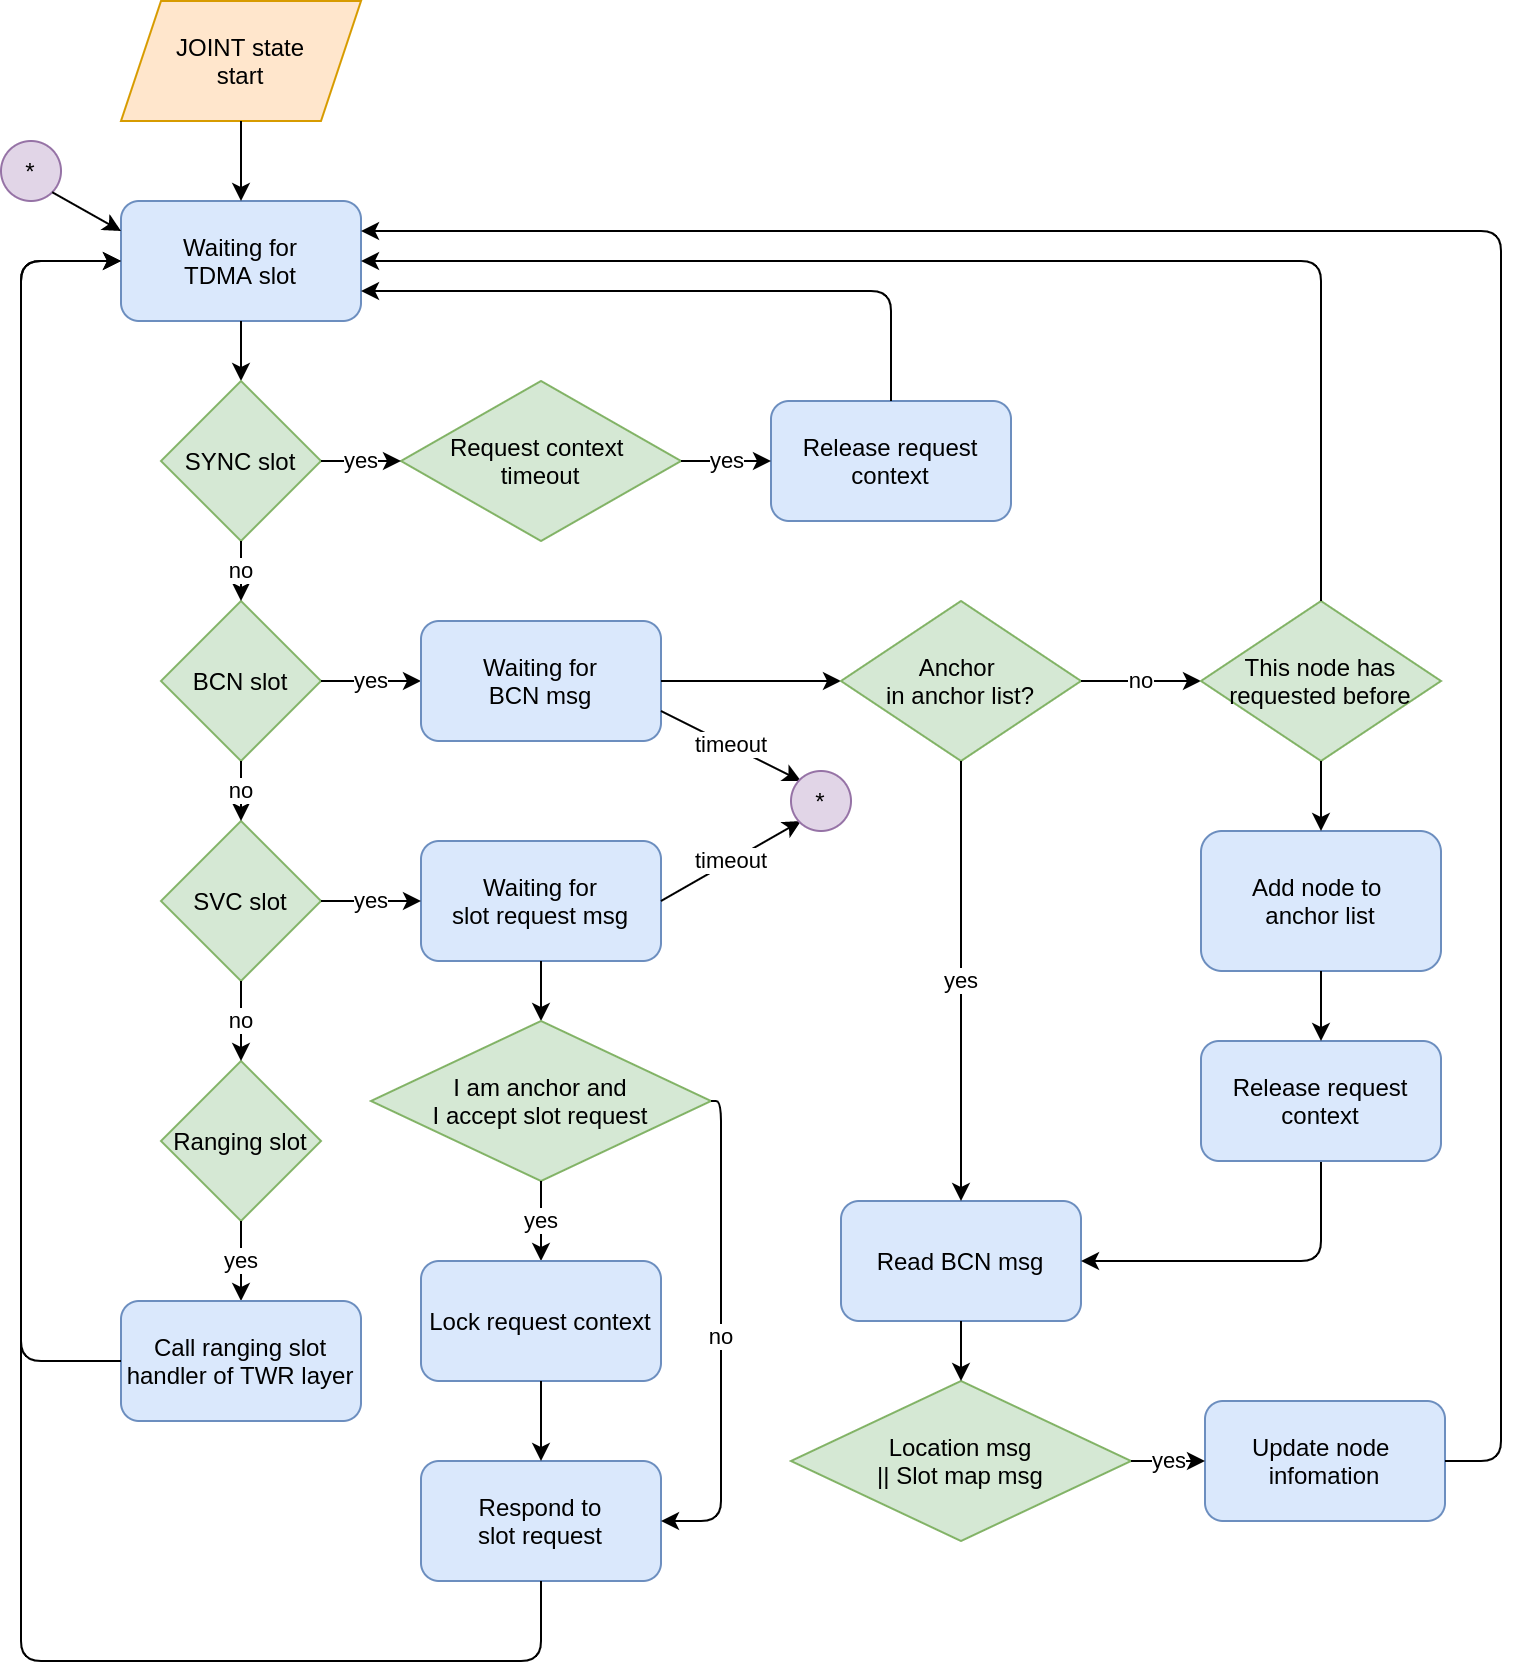
\includegraphics[scale=0.32]{JOINTED_state_flow_chart.png}
    \end{center}
    \caption{JOINTED state diagram}
    \label{fig:JOINTED_state_diagram}
\end{figure}

\section{Two way ranging (TWR)}
By using TWR, the need of synchronized clocks is eliminated since both the round-trip time(s) and the reply time(s) can be calculated separately using timestamps derived from each device.
\begin{figure}[H]
    \begin{center}
        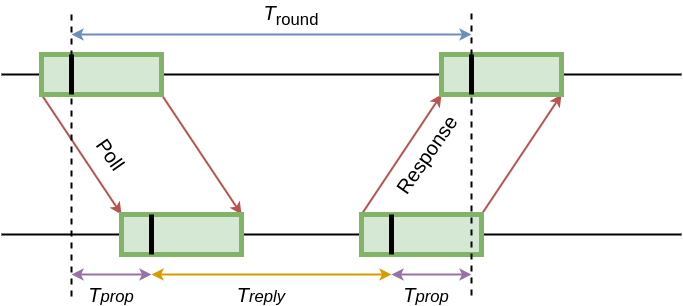
\includegraphics[scale=0.32]{single_sided_two_way_ranging.png}
    \end{center}
    \caption{Single-sided two-way ranging}
    \label{fig:single_sided_two_way_ranging}
\end{figure}
\end{document}